%
% TAZ.tex
%
% History of LulzBot Printers
%
% Copyright (C) 2014, 2015 Aleph Objects, Inc.
%
% This document is licensed under the Creative Commons Attribution 4.0
% International Public License (CC BY-SA 4.0) by Aleph Objects, Inc.
%

\section{LulzBot TAZ 1.0}
LulzBot TAZ 1.0.

\begin{figure}[h!]
\thisfloatpagestyle{empty}
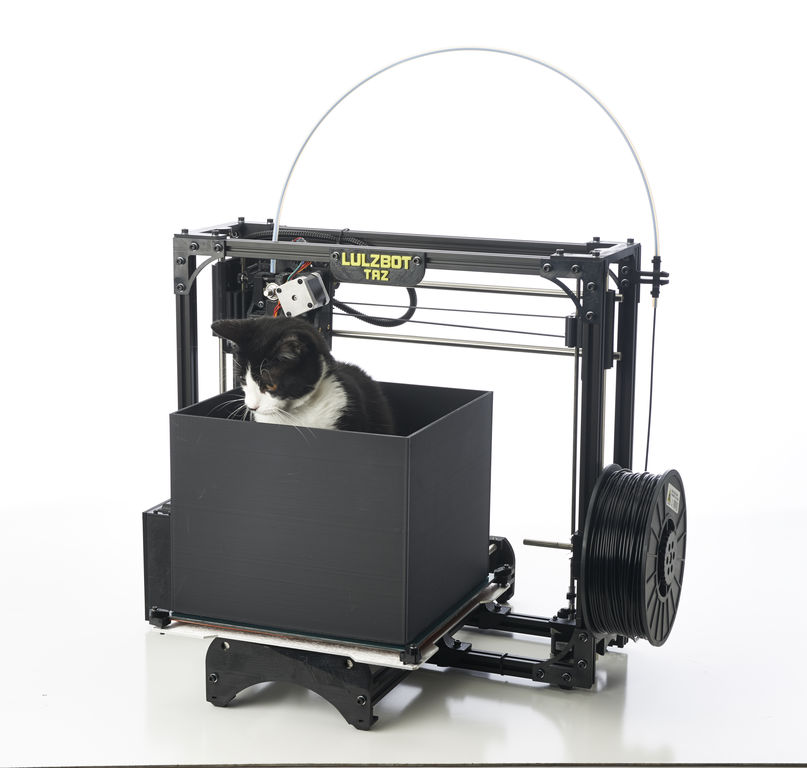
\includegraphics[keepaspectratio=true,height=0.40\textheight,width=1.00\textwidth,angle=0]{taz/taz-1-cat.jpg}
 \caption{LulzBot TAZ 1.0 with Cat.}
 \label{fig:taz-1-cat}
\end{figure}

\begin{figure}[h!]
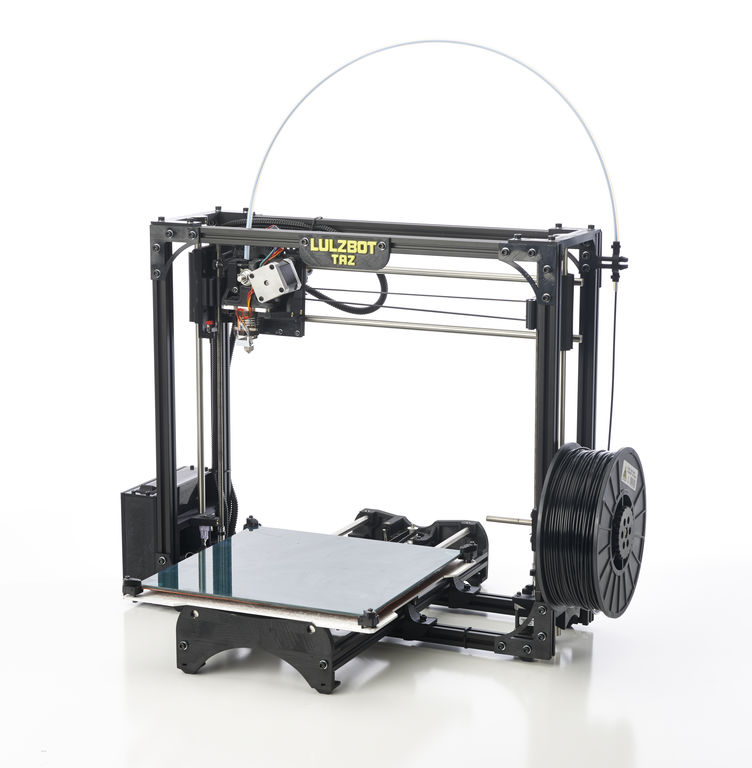
\includegraphics[keepaspectratio=true,height=0.40\textheight,width=1.00\textwidth,angle=0]{taz/taz-1.jpg}
 \caption{LulzBot TAZ 1.0.}
 \label{fig:taz-1}
\end{figure}

\begin{figure}[h!]
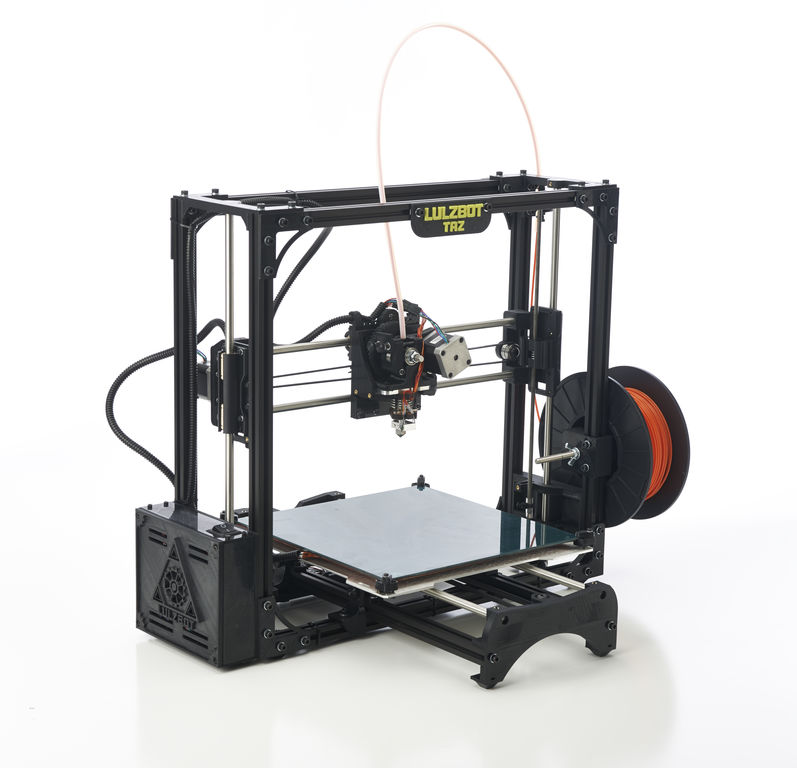
\includegraphics[keepaspectratio=true,height=0.40\textheight,width=1.00\textwidth,angle=0]{taz/taz-1-front-left.jpg}
 \caption{LulzBot TAZ 1.0 Front Left.}
 \label{fig:taz-1-front-left}
\end{figure}

\begin{figure}[h!]
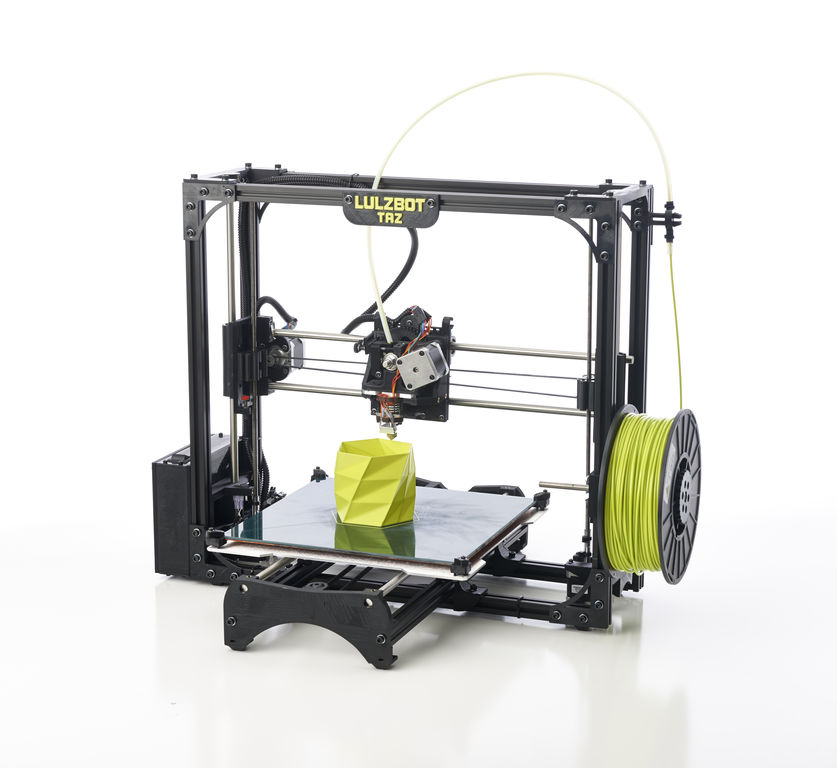
\includegraphics[keepaspectratio=true,height=0.40\textheight,width=1.00\textwidth,angle=0]{taz/taz-1-vase.jpg}
 \caption{LulzBot TAZ 1.0 with Vase.}
 \label{fig:taz-1-vase}
\end{figure}

\begin{figure}[h!]
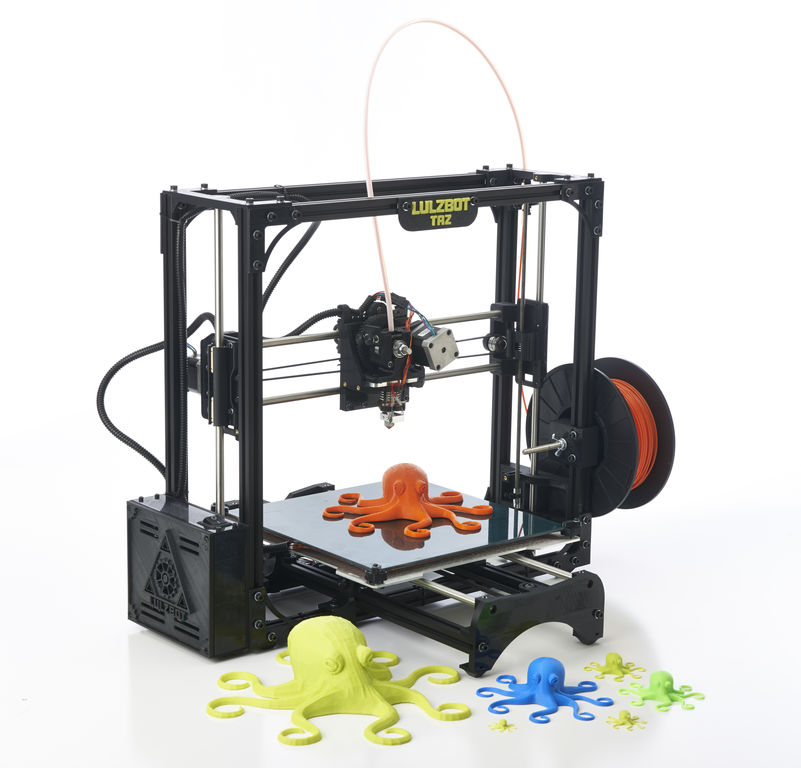
\includegraphics[keepaspectratio=true,height=0.40\textheight,width=1.00\textwidth,angle=0]{taz/taz-1-octo.jpg}
 \caption{LulzBot TAZ 1.0 with Octopus.}
 \label{fig:taz-1-octo}
\end{figure}

\begin{figure}[h!]
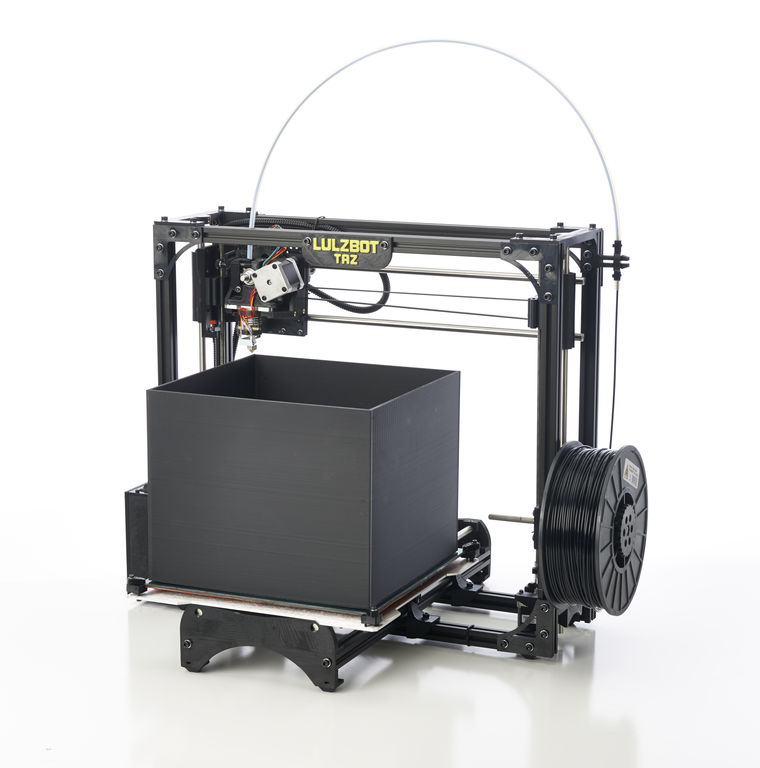
\includegraphics[keepaspectratio=true,height=0.40\textheight,width=1.00\textwidth,angle=0]{taz/taz-1-max.jpg}
 \caption{LulzBot TAZ 1.0 Max Build Volume.}
 \label{fig:taz-1-max}
\end{figure}
